\begin{center}
    \section*{\underline{Wechselstrom}}
\end{center}

\begin{tikzpicture}[remember picture, overlay]

% ---- ERSTE REIHE: Am Seitenursprung starten
\setlength{\rowheight}{28mm}

    % A1) Erste Kachel absolut platzieren
    \setlength{\cellwidth}{40mm}
    \Tile{A1}{([xshift=10mm,yshift=-20mm]current page.north west)}{\cellwidth}{\rowheight}
        {
            \vspace{-\TileSep}
            \titlerm{Grundgesetze}\\ \vspace{-2mm}
            \begin{equation*}
                u(t) = \hat u\cdot\sin(\omega\cdot t + \varphi_u)
            \end{equation*}
            \vspace{-2mm}
            \begin{equation*}
                i(t) = \hat i\cdot\sin(\omega\cdot t + \varphi_i)
            \end{equation*}
        }{0}{1}{1}{0}

    % B1) Zweite Kachel rechts anbauen
    \setlength{\cellwidth}{36mm}
    \Tile{B1}{(A1.north east)}{\cellwidth}{\rowheight}
        {
            \vspace{-\TileSep}
            \titlerm{(Kreis-) Frequenz}\\ \vspace{-2.5mm}
            \begin{equation*}
                \omega = 2\cdot\pi\cdot f = \frac{2\cdot\pi}{T}
            \end{equation*}
            \vspace{-2.5mm}
            \begin{equation*}
                f = \frac{1}{T}
            \end{equation*}
        }{0}{1}{1}{0}

    % C1) Dritte Kachel rechts anbauen
    \setlength{\cellwidth}{114mm}
    \Tile{C1}{(B1.north east)}{\cellwidth}{\rowheight}
        {
            \vspace{-\TileSep}
            \titlebf{Ohm'scher Widerstand}\\ \vspace{2mm}
            \begin{minipage}{0.32\cellwidth-\TileSep}
                \centering
                \titlerm{Ohm'sches Gesetz}\\ \vspace{-3mm}
                \begin{equation*}
                    u_\text{R}(t) = R\cdot i_R(t)
                \end{equation*}
                \vspace{-4mm}
                \begin{equation*}
                    \hat U_\text{R} = R\cdot\hat I_R
                \end{equation*}
                \vspace{-1mm}
            \end{minipage}%
            \vrule
            \begin{minipage}{0.37\cellwidth}
                \centering
                \titlerm{Phasenwinkel}\\ \vspace{-3mm}
                \begin{equation*}
                    \varphi_u = \varphi_i
                \end{equation*}
                \vspace{-4mm}
                \begin{equation*}
                    \varphi_\text{L} = \Delta\varphi = \varphi_u-\varphi_i = 0^\circ
                \end{equation*}
                \vspace{-1mm}
            \end{minipage}%
            \vrule
            \begin{minipage}{0.30\cellwidth-\TileSep}
                \centering
                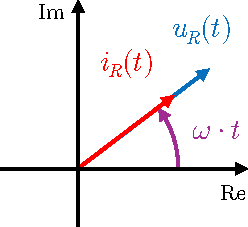
\includegraphics[width=0.67\textwidth]{images/phase-ohmscher-widerstand.pdf}
            \end{minipage}
        }{0}{0}{1}{0}

% ---- ZWEITE REIHE: unten anbauen
\setlength{\rowheight}{24mm}

    % X2) EIGENES FELD für Zeilenüberschrift
    \Tile{X2}{(A1.south west)}{190mm}{8mm}
        {
            \vspace{1mm}
            \titlebf{Induktivität einer Spule}
        }{0}{0}{0}{0}

    % A2) Erste Kachel unten anbauen
    \setlength{\cellwidth}{34mm}
    \Tile{A2}{(X2.south west)}{\cellwidth}{\rowheight}
        {
            \vspace{-\TileSep}
            \titlerm{Ideale Spule}\\ \vspace{-4mm}
            \begin{equation*}
                L \approx \mu_0\cdot\mu_\text{r}\cdot N^2\cdot\frac{A}{l}
            \end{equation*}
            \begin{equation*}
                u_\text{L}(t) = L\cdot\frac{\text{d}i_\text{L}(t)}{\text{d}t}
            \end{equation*}
        }{0}{1}{1}{0}

    % B2) Zweite Kachel rechts anbauen
    \setlength{\cellwidth}{48mm}
    \Tile{B2}{(A2.north east)}{\cellwidth}{\rowheight}
        {
            \vspace{-\TileSep}
            \titlerm{In Reihe- \& Parallel}\\ \vspace{-3.5mm}
            \begin{equation*}
                \text{Reihe: }L_\text{ges} = L_1 + L_2 + \dots
            \end{equation*}
            \begin{equation*}
                \text{Parallel: }\frac{1}{L_\text{ges}} = \frac{1}{L_1} + \frac{1}{L_2} + \dots
            \end{equation*}
        }{0}{1}{1}{0}

    % C2) Dritte Kachel rechts anbauen
    \setlength{\cellwidth}{64mm}
    \Tile{C2}{(B2.north east)}{\cellwidth}{\rowheight}
        {
            \vspace{-\TileSep}
            \titlerm{Spannung \& Strom}\\ \vspace{-4mm}
                \begin{align*}
                    u_\text{L}(t) &= \omega\cdot L\cdot i_\text{L}(t)\cdot\sin\!\left(\omega\cdot t\cdot\varphi_i + \tfrac{\pi}{2}\right) \\
                    i_\text{L}(t) &= \hat i_\text{L}\cdot \sin(\omega\cdot t + \varphi_i)
                \end{align*}
                \vspace{-4.5mm}
                \begin{equation*}
                    \hat u_\text{L} = \omega\cdot L\cdot\hat i_\text{L}
                \end{equation*}
        }{0}{1}{1}{0}

    % D2) Vierte Kachel rechts anbauen
    \setlength{\cellwidth}{44mm}
    \Tile{D2}{(C2.north east)}{\cellwidth}{\rowheight}
        {
            \vspace{-\TileSep}
            \titlerm{Phasenwinkel}\\ \vspace{-3mm}
                \begin{equation*}
                    \varphi_u = \varphi_i + \tfrac{\pi}{2}
                \end{equation*}
                \begin{equation*}
                    \varphi_\text{L} = \Delta\varphi = \varphi_u - \varphi_i = 90^\circ
                \end{equation*}
        }{0}{0}{1}{0}

% ---- DRITTE REIHE: unten anbauen
\setlength{\rowheight}{24mm}

    % X3) EIGENES FELD für Zeilenüberschrift
    \Tile{X3}{(A2.south west)}{190mm}{8mm}
        {
            \vspace{1mm}
            \titlebf{Kapazität eines Kondensators}
        }{0}{0}{0}{0}

    % A3) Erste Kachel unten anbauen
    \setlength{\cellwidth}{34mm}
    \Tile{A3}{(X3.south west)}{\cellwidth}{\rowheight}
        {
            \vspace{-\TileSep}
            \titlerm{Kondensator}\\ \vspace{-4mm}
            \begin{equation*}
                C \approx \epsilon_0 \cdot \epsilon_\text{r} \cdot\frac{A}{d}
            \end{equation*}
            \begin{equation*}
                i_\text{C}(t) = C\cdot\frac{\text{d}u_\text{C}(t)}{\text{d}t}
            \end{equation*}
        }{0}{1}{1}{0}

    % B3) Zweite Kachel rechts anbauen
    \setlength{\cellwidth}{48mm}
    \Tile{B3}{(A3.north east)}{\cellwidth}{\rowheight}
        {
            \vspace{-\TileSep}
            \titlerm{In Reihe- \& Parallel}\\ \vspace{-3.5mm}
            \begin{equation*}
                \text{Reihe: }\frac{1}{C_\text{ges}} = \frac{1}{C_1} + \frac{1}{C_2} + \dots
            \end{equation*}
            \begin{equation*}
                \text{Parallel: }C_\text{ges} = C_1 + C_2 + \dots
            \end{equation*}
        }{0}{1}{1}{0}

    % C3) Dritte Kachel rechts anbauen
    \setlength{\cellwidth}{64mm}
    \Tile{C3}{(B3.north east)}{\cellwidth}{\rowheight}
        {
            \vspace{-\TileSep}
            \titlerm{Spannung \& Strom}\\ \vspace{-4mm}
                \begin{align*}
                    u_\text{C}(t) &= \hat u_\text{C}\cdot\sin(\omega\cdot t + \varphi_u) \\
                    i_\text{C}(t) &= \omega\cdot C\cdot u_\text{C}(t)\cdot\sin\!\left(\omega\cdot t\cdot\varphi_u + \tfrac{\pi}{2}\right)
                \end{align*}
                \vspace{-4.5mm}
                \begin{equation*}
                    \hat i_\text{C} = \omega\cdot C\cdot\hat u_\text{C}
                \end{equation*}
        }{0}{1}{1}{0}

    % D3) Vierte Kachel rechts anbauen
    \setlength{\cellwidth}{44mm}
    \Tile{D3}{(C3.north east)}{\cellwidth}{\rowheight}
        {
            \vspace{-\TileSep}
            \titlerm{Phasenwinkel}\\ \vspace{-3mm}
                \begin{equation*}
                    \varphi_u = \varphi_i - \tfrac{\pi}{2}
                \end{equation*}
                \begin{equation*}
                    \varphi_\text{C} = \Delta\varphi = \varphi_u - \varphi_i = -90^\circ
                \end{equation*}
        }{0}{0}{1}{0}

% ---- VIERTE REIHE: unten anbauen
\setlength{\rowheight}{38mm}

    % X4) EIGENES FELD für Zeilenüberschrift
    \Tile{X4}{(A3.south west)}{190mm}{8mm}
        {
            \vspace{1mm}
            \titlebf{Zeigerdiagramme}
        }{0}{0}{0}{0}

    % A4) Erste Kachel unten anbauen
    \setlength{\cellwidth}{46mm}
    \Tile{A4}{(X4.south west)}{\cellwidth}{\rowheight}
        {
            \vspace{-\TileSep}
            \titlerm{Aufbau}\\ \vspace{2mm}
            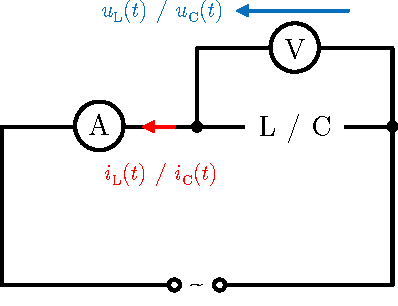
\includegraphics[width=\cellwidth-3\TileSep]{images/zeiger-aufbau.pdf}
        }{0}{1}{1}{0}

    % B4) Zweite Kachel rechts anbauen
    \setlength{\cellwidth}{72mm}
    \Tile{B4}{(A4.north east)}{\cellwidth}{\rowheight}
        {
            \vspace{-\TileSep}
            \titlerm{Spule}\\
            \hspace{1mm}
            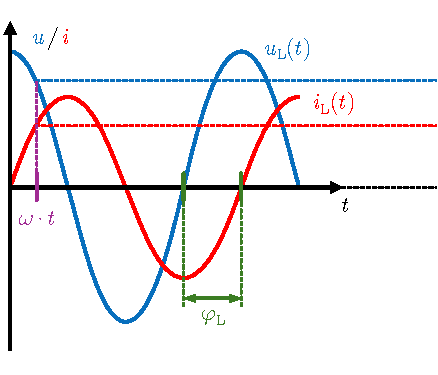
\includegraphics[height=33mm]{images/zeiger-diagramm-spule.pdf}
            \hspace{-8.15mm}
            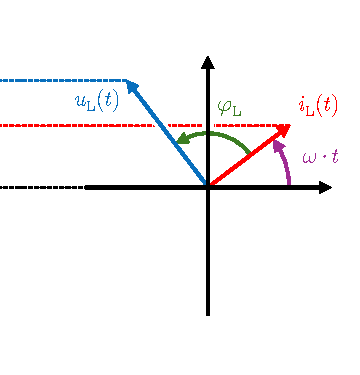
\includegraphics[height=33mm]{images/zeiger-ebene-spule.pdf}
        }{0}{1}{1}{0}

    % C4) Dritte Kachel rechts anbauen
    \setlength{\cellwidth}{72mm}
    \Tile{C4}{(B4.north east)}{\cellwidth}{\rowheight}
        {
            \vspace{-\TileSep}
            \titlerm{Kondensator}\\
            \hspace{1mm}
            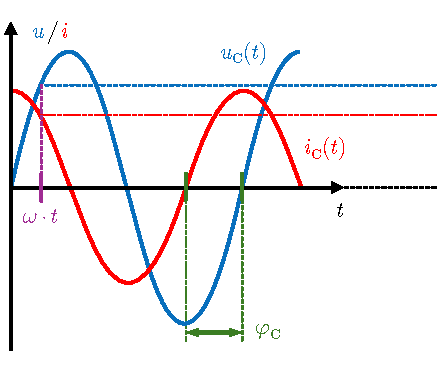
\includegraphics[height=33mm]{images/zeiger-diagramm-kondensator.pdf}
            \hspace{-8.35mm}
            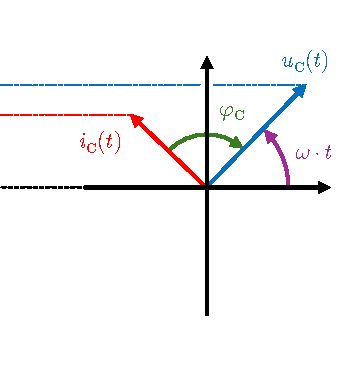
\includegraphics[height=33mm]{images/zeiger-ebene-kondensator.pdf}
        }{0}{0}{1}{0}

\end{tikzpicture}